\chapter{Denoising Autoencoder}

\indent\indent Denoising autoencoders are used to denoise an input image. They are widely used as first pre--processing step in various image processing applications. This chapter gives a brief introduction to denoising autoencoders. It further gives a description of our model summary and training details. 

\section{Autoencoding}
"Autoencoding" is a data compression algorithm where the compression and decompression functions are 1) data-specific, 2) lossy, and 3) learned automatically from examples rather than engineered by a human. These compression and decompression functions are usually implemented using neural networks.

\begin{enumerate}
\item Autoencoders are data-specific : they will only be able to compress data similar to what they have been trained on. An autoencoder trained on pictures of faces would do a rather poor job of compressing pictures of trees, because the features it would learn would be face-specific. Hence, one model cannot be generalised to all applications. They are application specific.
\item Autoencoders are lossy : the decompressed outputs will be degraded compared to the original inputs (similar to MP3 or JPEG compression). This differs from lossless arithmetic compression.
\item Autoencoders are learned automatically from data examples : it means that it is easy to train specialized instances of the algorithm that will perform well on a specific type of input. It doesn't require any new engineering, just appropriate training data.
\end{enumerate}
The aim of an autoencoder is dimensionality reduction and feature discovery. An autoencoder is trained to predict its own input,
but to prevent the model from learning the identity mapping,
some constraints are applied to the hidden units.\cite{yasenko2020image}
\vspace{0.75cm}

\section{\gls{da}}
Denoising autoencoders are an extension of simple autoencoders.  They add noise to inputs during a training process. Autoencoders are one of the unsupervised deep learning models. \cite{yasenko2020image} \\
Algorithm of \acrshort{da}:
\begin{enumerate}
    \item Manually adding noise, for our project, Gaussian Blur.
    \item Constructing an autoencoder model. It includes both encoding and decoding layers for compression and decompression respectively.
    \item Training the denoising autoencoder model on the noisy dataset. The reconstruction loss between the original image and its reconstruction obtained from final decoding layer is minimised in every epoch.
\end{enumerate}

% \ref{fig:autoencoder_schema} 
\begin{figure}[htb]
\centering
	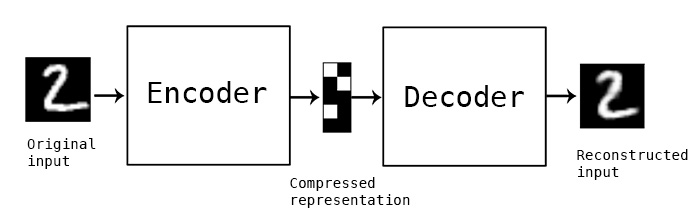
\includegraphics[scale=2.5]{Figures/autoencoder_schema}	
	\caption{Denoising Autoencoder}
	\label{fig:autoencoder_schema}
\end{figure}
\section{Software Setup}
\begin{enumerate}
\item Keras: Keras is an open-source software library that provides a python interface for artificial neural networks. Keras acts as an interface for the TensorFlow library.
\item PyCharm: PyCharm is an integrated development environment used in computer programming, specifically for the Python language.
\item Google Colab: Colaboratory, or “Colab” for short, is a product from Google Research. Colab allows anybody to write and execute arbitrary python code through the browser, and is especially well suited to machine learning, data analysis and education.
\end{enumerate}
\section{\gls{da} model summary}

% \ref{fig:denoise_model_summary} 
\begin{figure}[H]
\centering
	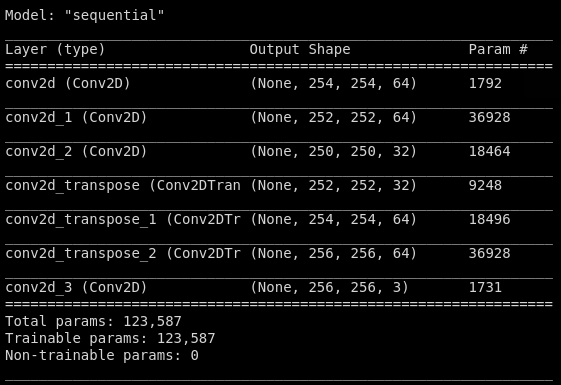
\includegraphics[scale=0.7]{Figures/denoise_model_summary.png}	
	\caption{Model Summary of \acrlong{da}}
	\label{fig:denoise_model_summary}
\end{figure}

\section{Training details}
The model is developed and trained using Keras framework with Tensorflow backend. The model has three convolution layers for encoding or compressing and three convolution transpose layers i.e. convolution $+$ upsampling, for decoding or decompressing as shown in figure \ref{fig:denoise_model_summary}. The last convolution layer is used to map the normalised pixel values between 0 and 1. To achieve this, sigmoid activation function is used which is given by \ref{c4:eqn1}.\\
% Choice of activation function and loss function:\\ 
% Sigmoid activation function is used in the last convolution layer to map the normalised pixel values to a value between 0 and 1. \\
% Sigmoid activation function is given by \ref{c4:eqn1}. 
\begin{equation}
\label{c4:eqn1}
\fontsize{12}{12}\selectfont
f(s_{i}) = \frac{1}{(1+e^{x})}
\end{equation}
% \ref{fig:Sigmoid} 
\begin{figure}[H]
\centering
	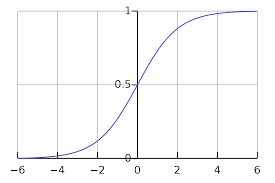
\includegraphics[scale=1]{Figures/sigmoid.png}	
	\caption{Sigmoid activation function}
	\label{fig:Sigmoid}
\end{figure}
The reconstruction loss is calculated for these mapped values using Binary Cross-Entropy Loss function (Sigmoid Cross-Entropy loss function), which is given by equations \ref{c4:eqn2} and \ref{c4:eqn3}.
\begin{equation}
\label{c4:eqn2}
\fontsize{12}{12}\selectfont
\begin{aligned}
\gls{ce} 
& = \sum_{i=1}^{c'=2}{(t_{i})\log(f(s_{i})))}\\
& = -{(t_{1})\log(f(s_{1}))} - ({1 - (t_{1}))\log(1 - f(s_{1}))}
\end{aligned}
\end{equation}

\begin{equation}
\label{c4:eqn3}
\fontsize{12}{12}\selectfont
\gls{ce} = 
\begin{cases}
  -\log(f(s_{1})) & if \hspace{5pt} t_{1} = 1 \\
  -\log(1 - f(s_{1})) & if \hspace{5pt} t_{1} = 0\\
\end{cases}
\end{equation}

To summarize, a denoising autoencoder is an image processing technique which is used to remove noise from an image. It has both downsampling and upsampling layers. In downsampling the model learns various features of the image and it reconstructs the image based on the learnt features in upsampling.

\begin{figure}[H]
\centering
	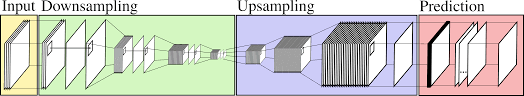
\includegraphics[scale=0.9]{Figures/denoise_summary.png}	
	\caption{\acrlong{da} summary}
	\label{fig:denoise_model_summary}
\end{figure}